\documentclass{jlreq}

\usepackage{bm}
\usepackage{fancyhdr}
\usepackage{float}
\usepackage{graphicx}

\pagestyle{fancy}
\fancyhf{}
\fancyhead[R]{\thepage}

\renewcommand\thesubsection{(\alph{subsection})}

\title{言語処理プログラミング 課題1}
\author{22122502 川口 栄宗}
\date{提出日: \today}

\begin{document}

\maketitle
\clearpage

\section{作成したプログラムの設計情報}

\subsection{全体構成}
モジュールの関係を図\ref{fig:module_map}に示す.

\begin{figure}
  \centering
  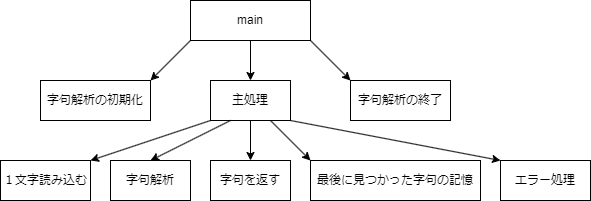
\includegraphics[width=\textwidth]{assets/lpp01_module.png}
  \caption{モジュール構成図}
  \label{fig:module_map}
\end{figure}

\subsection{各モジュールごとの構成}
\subsubsection{字句解析の初期化}

\subsubsection{主処理}
\subsubsection{字句解析の終了}

\subsection{各関数の外部(入出力)使用}

\section{テスト情報}

\subsection{テストデータ}
\subsection{テスト結果}
\subsection{テストデータの十分性}

\section{課題のスケジュールと実際の進捗状況}

\subsection{事前計画}
\subsection{実際の進捗状況}
\subsection{当初の事前計画と実際の進捗との差の原因}

\end{document}